%Space out the vacuum bra/ket a bit
\def \vacr {{\lvert\mkern1.5mu0\mkern1.5mu\rangle}}
\def \vacl {{\langle\mkern1.5mu0\mkern1.5mu\rvert}}

\chapter{The Standard Model of particle physics}\label{chap:SM}



The Standard Model (SM) of particle physics is a quantum field theory (QFT) with multiple interacting fields and symmetries. It was developed during the second half of the $20^{\mathrm{th}}$ century. There has been excellent agreement between the predictions of the SM and experimental data from particle physics experiments. An overview of the standard model is presented in \cref{sec:SM:intro}. The SM Lagrangian is described in \cref{sec:SM:lagrangian}, outlining each of its components.

Natural units are used throughout this thesis, where $\hbar=h/2\pi=c=1$ is used. Therefore, masses and momenta are quoted in unites of energy, electron volts (\SI{}{\electronvolt}). 
% An Examples is the predicted magnetic dipole moment of an electron agrees with the measured value to a very high precision. Further verifications of the SM include the discovery of the Top quark by CDF and D$\emptyset$ experiments at the Tevatron \protonproton collider~\cite{Abe1995,Abachi1995}. The tau neutrino~\cite{Kodama_2001} in 2009. The most recent validation of the SM was via the observation of the Higgs Boson by the ATLAS and CMS experiments at the LHC in 2012~\cite{Chatrchyan2012,Aad_2012}. This chapter will give an introduction to the Standard Model of particle physics and its interactions. The strong, electroweak and Higgs interactions are also discussed. 
\section{Introduction}
\subsubsection{Fundamental mathematical concepts}
The mathematical structure of the SM is given by a gauge quantum field theory~\cite{Peskin1995}. In both classical and quantum field theory, the dynamics of a system are described by the Lagrangian density, which henceforth will be referred to simply as the Lagrangian. Consider the Lagrangian for a massive complex field, $\psi$, with mass, $m$, 
\begin{equation}
    \label{eq:lagrangian_example}
    \begin{aligned}
        & \mathcal{L} = \partial^\mu\bar{\psi}\partial_\mu\psi - m\bar{\psi}\psi,
    \end{aligned}
\end{equation}
where the first term is referred to as the kinetic term and the second term is the mass term of the field. The Lagrangian can be used to calculate the scattering amplitudes of reactions using well-defined methods~\cite{Lehmann1955} and the interactions can be expressed in terms of diagrams known as Feynman diagrams~\cite{Thomson:2013zua}. The use of Feynman diagrams simplifies the process of calculation of the scattering amplitudes.

In natural units, all quantities are measured in units of powers of energy. For example, $[m] = E^1$, where $[m]$ corresponds to the dimensionality of $m$. The fundamental quantity in mechanics is the action, $S$, the time integral of a Lagrangian~\cite{Peskin1995}
\begin{equation}
    \label{eq:action}
    \begin{aligned}
        & S = \int \mathcal{L}~d^4x.
    \end{aligned}
\end{equation}
The principle of least action states that when a system evolves from one configuration to another with a given time, it does so along the \emph{path} for which $S$ is a minimum. The action is dimensionless, therefore the Lagrangian has dimensionality $[\mathcal{L}] = E^4$.

Symmetries are central to our current understanding of particle physics. In particle physics, a symmetry of the universe is expressed by requiring that all physical predictions are unchanged or invariant under the same set of transformations. The importance of the concept of symmetries originates from Noether's theorem~\cite{Noether1918}, stipulating that for every continuous symmetry there is a corresponding conservation law. In the context of field theory, one of the cornerstones in the construction of the SM is the notion of gauge symmetry. The Lagrangian defined in \cref{eq:lagrangian_example} is invariant with respect to rotation with angle $\alpha$ in the complex plane 
\begin{equation}
    \label{eq:unitary}
    \begin{aligned}
        \psi(x) \rightarrow \psi(x)e^{i\alpha}~,~\bar{\psi}(x) \rightarrow \bar{\psi}e^{-i\alpha}.
    \end{aligned}
\end{equation}
Therefore, it can be said that the Lagrangian is invariant under global one-dimensional unitary transformations, $\mathrm{U(1)}$, where global denotes that $\alpha$ is the same for any value of $x$~\cite{stephanhaywood}. However, if $\alpha$ depends on $x$ the $\mathrm{U(1)}$ symmetry is broken. Hence, the Lagrangian is not invariant under a local $\mathrm{U(1)}$ transformation. The required gauge invariance can be restored by replacing the derivative in \cref{eq:lagrangian_example} with a \emph{covariant} derivative, $D_\mu$, defined as 
\begin{equation}
    \label{eq:covdir}
    \begin{aligned}
        D_\mu = \partial_\mu + iqA_\mu(x),
    \end{aligned}
\end{equation}
where $A_\mu(x)$ is a new field that transforms as $A_\mu \rightarrow A_\mu - \frac{1}{q}\partial_\mu\alpha(x)$ and $q$ is the coupling strength between the field $\psi$ and $A_\mu$. Therefore, the Lagrangian is now invariant under local $\mathrm{U(1)}$ transformation. The introduced field, $A_\mu$, is known as a \emph{gauge field}, and the Lagrangian under these modifications is known as a \emph{gauge theory}. The number of gauge fields required to restore a given local symmetry is related to the number of generators in the symmetry group, for example, $\mathrm{U(1)}$ is a symmetry group with one generator, which results in the addition of a single gauge field. 

\subsubsection{Overview of Standard Model}\label{sec:SM:intro}
The SM is a gauge theory that describes the elementary particle and their fundamental interactions (excluding gravity). Interactions of the SM are considered in terms of fields, $\psi$, of half-integer spin fermions and integer spin gauge bosons, $\phi$. The fermions consist of 12 particles (with their corresponding anti-particles) in total classified into quarks and leptons. The gauge bosons mediate the fundamental forces between the fermions. The SM describes three fundamental forces: the electromagnetic, the weak, and the strong interaction. The different properties (mass, charge and spin) of the SM particles are summarised in \cref{fig:sm_diagram}. 

The full gauge symmetry group of the SM is given by $\mathrm{SU(3)}_\mathrm{C} \otimes \mathrm{SU(2)}_\mathrm{L} \otimes \mathrm{U(1)}_\mathrm{Y}$, where $\mathrm{SU(n)}$ is a special unitary group with $n$ dimension~\cite{stephanhaywood}. The indices C, L, Y represent the \emph{colour} (strong interaction), \emph{weak isospin} and \emph{weak hypercharge} (both electroweak interactions), respectively. The electroweak theory unifies the electromagnetic and weak interactions and is based on the conservation of electric charge, Q, which is convolved with the weak isospin and hypercharge (described in \cref{sec:SM:lagrangian}). The description of the strong interaction is based on the theory of Quantum Chromodynamics (QCD)~\cite{Zweig:1964jf}. The conserved quantity in QCD is the colour charge (C), and it is represented by three possible colours: for example these could be red, green, and blue. 

\begin{figure}[!htpb]
    \centering
    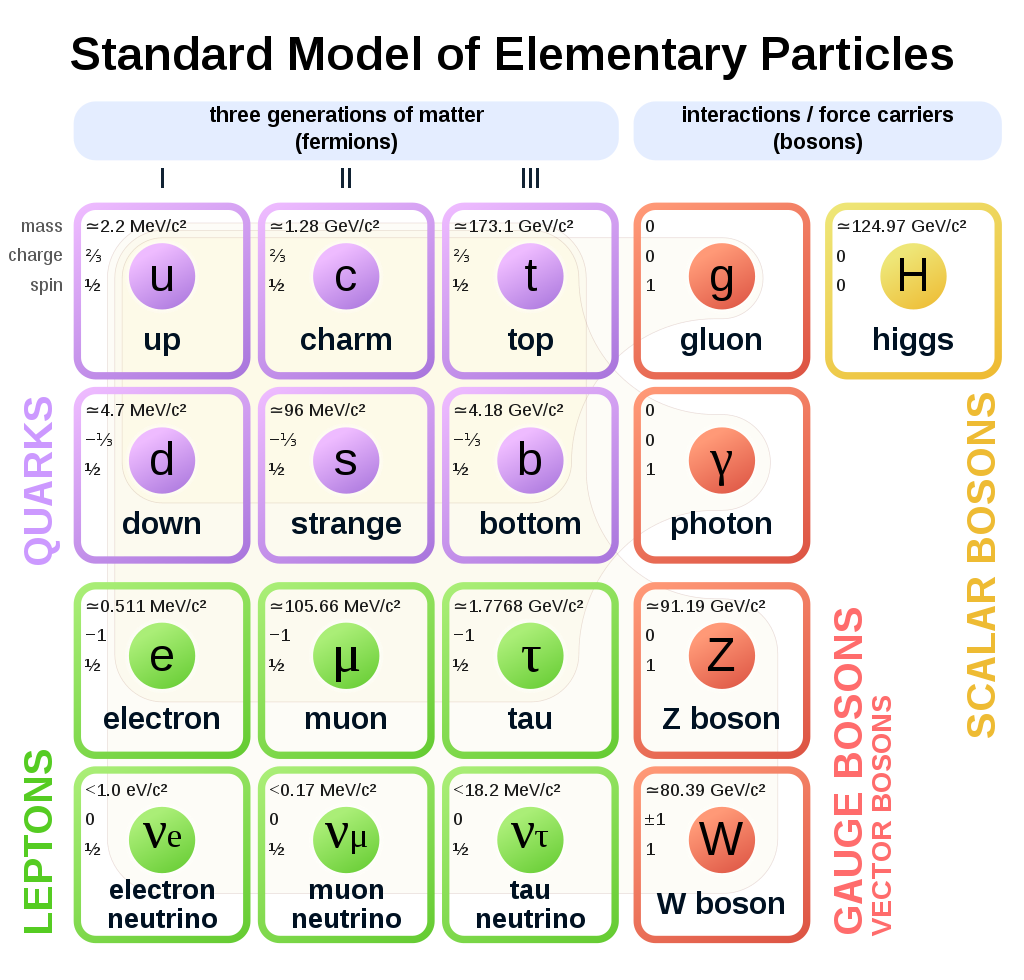
\includegraphics[width=0.8\textwidth]{/Users/Deshan/Documents/PhD/thesis/Thesis/figures/theory/sm/SM_diagram.png}
    \caption{Overview of the fundamental fermions and bosons in the Standard Model. The mass, charge and spin of each particle is given~\cite{wiki:xxx}.}
    \label{fig:sm_diagram}
\end{figure}

\section{The standard model Lagrangian}\label{sec:SM:lagrangian}
The SM can be expressed by the following Lagrangian
\begin{equation}
    \label{eq:lagrangianSM}
    \begin{aligned}
        & \mathcal{L}_\mathrm{SM} = \mathcal{L}_\mathrm{Fermions} + \mathcal{L}_\mathrm{Gauge} + \mathcal{L}_\mathrm{Higgs} + \mathcal{L}_\mathrm{Yukawa}.
    \end{aligned}
\end{equation}
The following sections will review each of the components of the SM Lagrangian. These sections are based on ~\cite{Thomson:2013zua,Peskin:1995ev}.

\subsection{Fermion fields}\label{sec:fermionFields}
The first component of the Lagrangian in \cref{eq:lagrangianSM} describes the propagation and interactions of fermions. There are three generations of particles observed in the fermion sector, where each generation has the same fundamental properties except for the different masses. The fermions can be categorised into three distinct types: Weyl, Dirac and Majorana. Weyl fermions are massless, Dirac fermions are massive, and Majorana fermions are particles that are the same as their antiparticle. In the SM, fermions are considered to be Dirac fermions, with the exception of neutrinos, as their nature is not yet determined to be Dirac or Majorana. 

The quark fields are represented as colour triplets transforming with the corresponding representation of SU(3). Whereas, the lepton fields are colourless, which results in them not being charged under the strong interaction. Therefore, fermions are categorised into families of particles that interact via the strong interaction and ones that do not, and these are termed quarks and leptons, respectively. Each lepton generation contains an electrically-charged particle and one which has neutral charge. The quark generations are split into up-type and down-type quarks that have an electric charge of $+\frac{2}{3}$ and $-\frac{1}{3}$, respectively. 

An individual fermion field can be described by the following Dirac Lagrangian
\begin{equation}
    \label{eq:lagrangianFermion}
    \begin{aligned}
        & \mathcal{L}_\mathrm{Fermion} = \bar{\psi}\left(i\gamma^\mu \partial_\mu - m\right)\psi,
    \end{aligned}
\end{equation}
where $\gamma^{\mu}$ are the Dirac matrices~\cite{doi:10.1098/rspa.1928.0023}. Imposing gauge invariance under SU(2)$_\mathrm{L}$ and U(1)$_\mathrm{Y}$ rotations, the Dirac Lagrangian can be written in terms of the covariant derivative, $D_\mu$, where the partial derivatives are replaced by the covariant derivative. The full description of the covariant derivative describing the interaction of the fermion field with the gauge field is given in \cref{sec:gaugeFields}. 

The distinction between \emph{left-handed} and \emph{right-handed} fermions are made in the SM. The left-handed fermions are grouped into weak isospin doublets with $T = \frac{1}{2}$, and the right-handed fermions are grouped into weak isospin singlets with $T = 0$, where $T$ is the weak isospin. 

In the Lagrangian for the electroweak unification, the weak hypercharge, $Y$, is defined in terms of the electric charge $Q$ and the third component of the weak isospin $T^3$ by the equation
\begin{equation}
    \label{eq:hypercharge}
    \begin{aligned}
        & Y = 2Q - 2T^3.
    \end{aligned}
\end{equation}
This results in $Y = -1, -\frac{1}{3}$ for the weak isospin doublets and $Y = -2,\frac{4}{3},-\frac{2}{3}$ for the weak isospin singlets. \cref{tab:fermions} shows the quantum numbers of the generations of both left- and right-handed fermions under the electroweak symmetry group. A consequence of the left-handed doublets and the right-handed singlets is that the Dirac mass terms for the fermion fields are not gauge invariant under the SU(2)$_\mathrm{L} \otimes \mathrm{U}(1)_\mathrm{Y}$ transformations. Therefore an alternative mechanism is needed to impose gauge invariance. The alternative mechanism will be introduced in \cref{sec:symmbreak}. The right-handed neutrinos are often omitted from the construction of the SM, as they have not yet been observed experimentally, but appear in many models for generating the experimentally-observed neutrino mass~\cite{Ahmad2002}.

\begin{table}[htp]
    \centering
    {
    \begin{tabular}{l | c c c | c c c c}
    \toprule
      & \multicolumn{3}{c|}{Generation} &  \multicolumn{4}{c}{Quantum Numbers}  \\
      & 1 & 2 & 3 & $T$ & $T^3$ & $Q$ & $Y$ \\ 
    \hline
    \multirow{4}{*}[0.5em]{quarks} & $u_L$ & $c_L$ & $t_L$ & $\frac{1}{2}$ & +$\frac{1}{2}$ & +$\frac{2}{3}$ & +$\frac{1}{3}$ \\
    & $d_L$ & $s_L$ & $b_L$ & $\frac{1}{2}$ & -$\frac{1}{2}$ & -$\frac{1}{3}$ & -$\frac{1}{3}$ \\
    & $u_R$ & $c_R$ & $t_R$ & $ 0$ & $0$ & +$\frac{2}{3}$ & +$\frac{4}{3}$ \\
    & $d_R$ & $s_R$ & $b_R$ & $ 0$ & $0$ & -$\frac{1}{3}$ & -$\frac{2}{3}$ \\
    \midrule
    \multirow{4}{*}[0.5em]{leptons} & $\nu_{e,L}$ & $\nu_{\mu,L}$ & $\nu_{\tau,L}$ & $\frac{1}{2}$ & +$\frac{1}{2}$ & +1 & 0 \\
    & $\nu_{e,R}$ & $\nu_{\mu,R}$ & $\nu_{\tau,R}$ & 0 & 0 & 0 & 0 \\
        & $e_R$ & $\mu_R$ & $\tau_R$ & $\frac{1}{2}$ & +$\frac{1}{2}$ & -1 & -1 \\
        & $e_L$ & $\mu_L$ & $\tau_L$ & 0 & 0 & -2 & -1 \\
    \bottomrule
    \end{tabular}
    }
    \caption{List of Standard Model fermions and their properties. The quantum numbers for the left (L) and right (R) fermions are given; weak isospin ($T$) with its third component $T^3$, hypercharge (Y) and charge (Q).}
    \label{tab:fermions}
\end{table}

\subsection{Gauge fields}\label{sec:gaugeFields}
The second component of the SM Lagrangian, $\mathcal{L}_{\mathrm{Gauge}}$, describes the propagation of gauge bosons. The gauge field Lagrangian is given by
\begin{equation}
    \label{eq:lagrangianGauge}
    \begin{aligned}
        & \mathcal{L}_\mathrm{Gauge} = -\frac{1}{4}G^a_{\mu\nu}G_a^{\mu\nu} -\frac{1}{4}W^a_{\mu\nu}W_a^{\mu\nu} -\frac{1}{4}B_{\mu\nu}B^{\mu\nu},
    \end{aligned}
\end{equation}
where the fields correspond to transformations of their respective symmetry groups, $B_\mu$ are the gauge fields corresponding to the U(1)$_\mathrm{Y}$ transformation,  $W_\mu^a$ with $a = 1,2,3$ corresponds to the SU(2)$_\mathrm{L}$ transformation and $G_\mu^a$ with $a = 1,..,8$ corresponds to the transformations under SU(3)$_\mathrm{C}$. 

The differences between these fields are a result of the different nature of the corresponding symmetry groups. Self-interactions between the $W_\mu$ and $G_\mu$ gauge fields are possible due to the non-abelian nature of the SU(2)$_\mathrm{L}$ and SU(3)$_\mathrm{C}$ groups. Whereas, due to the abelian nature of the U(1)$_\mathrm{Y}$ group, self-interactions between the fields are not possible.  

As mentioned in \cref{sec:fermionFields}, a covariant derivative, $D_\mu$, is defined to describe the coupling between the fermion fields and gauge fields. The full covariant derivative for a fermion interacting with all three fields (e.g. quarks) is defined as
\begin{equation}
    \label{eq:covaariantDerv}
    \begin{aligned}
        & D_\mu \psi = \left(\partial_\mu - ig_s\frac{\lambda_a}{2}G^a_\mu - igT_aW^a_\mu - ig^\prime YB_\mu\right)\psi,
    \end{aligned}
\end{equation}
where $g^\prime$, $g$ and $g_s$ are the coupling constants of the U(1)$_\mathrm{Y}$, SU(2)$_\mathrm{L}$ and SU(3)$_\mathrm{C}$ interactions, respectively. The terms $\lambda_a$, $T_a$ and $Y$ are the generators of the respective fields. The SU(3)$_\mathrm{C}$ gauge field is omitted for fermions that do not interact via the strong force. Therefore, the partial derivatives in the Dirac lagrangian is replaced, and the interactions for the electroweak and QCD components can be determined. 

\subsubsection{The electroweak interaction}\label{sec:electroweak}
Historically the electromagnetic and weak interactions were developed separately. The electromagnetic force is mediated by massless photons that propagate over an infinite range. The photons can interact with any particles which carry an electrical charge. The theory that describes the electromagnetic interaction is Quantum Electrodynamics (QED). The weak nuclear interaction acts on short length and time scales due to the large mass of its force carriers ($W^{\pm}$ and $Z$). Whereas, the weak bosons interact with left-handed fermions carrying a weak isospin quantum number. The weak force has two types of interactions: a charged current and a neutral current interaction. 

The unification of the two theories, the electroweak theory was developed by Glashow, Salam and Weinberg et al.~\cite{Glashow1959,Salam1959,Weinberg1967}. As a result, the electroweak theory is sometimes also referred to as the \emph{GSW} theory. The electroweak interactions are described by the SU(2)$_\mathrm{L}\otimes\mathrm{U(1)}_\mathrm{Y}$ symmetry group. The requirement for gauge invariance under these two symmetry groups leads to the following Lagrangian
\begin{equation}
    \label{eq:lagrangianEW}
    \begin{aligned}
        & \mathcal{L}_\mathrm{EW} = \bar{\psi}\slashed{D}\psi - \frac{1}{4}W^a_{\mu\nu}W_a^{\mu\nu} - \frac{1}{4}B_{\mu\nu}B^{\mu\nu},
     \end{aligned}
\end{equation}
where $\slashed{D} = \gamma^\mu D_\mu$, and is the covariant derivative with the SU(3)$_\mathrm{C}$ gauge fields omitted. The physical mass eigenstates of the charged $W^\pm_\mu$ fields can be obtained via a linear combination of $W^1_\mu$ and $W^2_\mu$. The mass eigenstates of the $Z$ boson field, $Z_\mu$, and the photon field, $A_\mu$ is obtained via rotations of the fields $W_\mu^3$ and $B_\mu$ around the weak mixing angle, $\theta_W$, to give
\begin{equation}\renewcommand*{\arraystretch}{\newarraystrech}
    \label{eq:wbosonFields}
    \begin{aligned}
        & W^\pm_\mu = \frac{1}{2} \left(W^1_\mu + W^2_\mu \right), \\
     \end{aligned}
\end{equation}
and 
\begin{equation}\renewcommand*{\arraystretch}{\newarraystrech}
    \label{eq:zbosonFields}
    \begin{aligned}
        & \begin{pmatrix}
            A_\mu \\*[0.6cm]
            Z_\mu
        \end{pmatrix} = \begin{pmatrix}
            \cos \theta_W & \sin \theta_W \\*[0.4cm]
            -\sin \theta_W & \cos \theta_W
        \end{pmatrix} \begin{pmatrix}
            B_\mu \\*[0.6cm]
            W_\mu^3
        \end{pmatrix}.
     \end{aligned}
\end{equation}
Experimental results have confirmed the existence of the $W^\pm$ and $Z$ bosons, with masses of $m_W = 80.379 \pm 0.012$ and $m_Z = 91.188 \pm 0.002$ \SI{}{\giga\electronvolt}, respectively~\cite{PDG}. However, the inclusion of the boson and fermion mass terms in the SM Lagrangian violates the SU(2)$_\mathrm{L} \otimes \mathrm{U(1)}_\mathrm{Y}$ symmetry, resulting in a non-normalisable theory. Therefore, this requires the introduction of the theory of spontaneous symmetry breaking, commonly known as the Higgs mechanism (\cref{sec:symmbreak}).

\subsubsection{Quantum Chromodynamics}
The SU(3)$_\mathrm{C}$ symmetry group corresponds to the strong nuclear force, and its interactions are described by Quantum Chromodynamics (QCD). Much of the structure and notation of the resulting gauge interactions have already been discussed. However, there are significant differences that are a result of the SU(3)$_\mathrm{C}$ group. The couplings between the quarks and gluons are defined from the SU(3)$_\mathrm{C}$ symmetry group, where colour charge is the conserved quantity. As a result of the eight generators of SU(3)$_\mathrm{C}$ there are eight associated gauge bosons (gluons). The gluons are colour charged, massless and have no electric charge. The Lagrangian for the quark interactions can be written as
\begin{equation}
    \label{eq:lagrangianQuark}
    \begin{aligned}
        & \mathcal{L}_\mathrm{Quark} = \frac{g_s}{2}\bar{\psi}_q \left(\gamma_\mu \lambda_a G_\mu^a \right)\psi_q ,
     \end{aligned}
\end{equation}
where $g_s$ is the coupling constant of the strong interaction and $G_\mu^a$ corresponds to the gluon field strength tensor. The coupling constant, $g_s$, is expressed as $\alpha_s = \frac{g_s^2}{4\pi}$ for convenience, and is a fundamental parameter of QCD, along with the quark masses. Using the QCD parameters, a scattering amplitude in a reaction between the initial and final state particles can be evaluated in powers of $\alpha_s$. However, in QFT there will be ultraviolet (UV) divergences that are a result of Feynman diagrams containing loops. The divergences need to be fixed using a renormalisation procedure, which involves including a scale, $\mu_R$, above which the UV divergences are removed. 

The dependence of the strength of the coupling on the scale ($Q^2$) is derived using the renormalisation group equation (RGE)~\cite{PDG}, which is expressed as
\begin{equation}
    \label{eq:rge}
    \begin{aligned}
        & Q^2 \frac{\partial\alpha_s}{\partial Q^2} = \beta(\alpha_s) = -\beta_0\alpha_s^2(1+\beta_1\alpha_s + \beta_2\alpha_s^2+ ..),
     \end{aligned}
\end{equation}
where $\beta_0 = (33-2n_f)/(12\pi)$ is known as the 1-loop $\beta$ function coefficient and $n_f$ denotes the number of quark flavours. \cref{fig:alphasrun} depicts the dependence of $\alpha_s$ on energy scale. This defines the characteristic properties of the QCD interactions: \emph{asymptotic freedom} and \emph{quark confinement}. As $Q^2$ increases the coupling of the strong interaction tends to zero. This process is known as asymptotic freedom, and it is observed experimentally, as shown in \cref{fig:alphasrun}. However, as $Q^2$ gets smaller, the coupling between the quarks becomes stronger and prevents them from existing as isolated particles. This phenomenon is known as quark confinement. The increase in potential energy as $Q^2$ increases is significant enough to create quark and anti-quark pairs in a process known as \emph{hadronisation}.
\begin{figure}[!htpb]
    \centering
    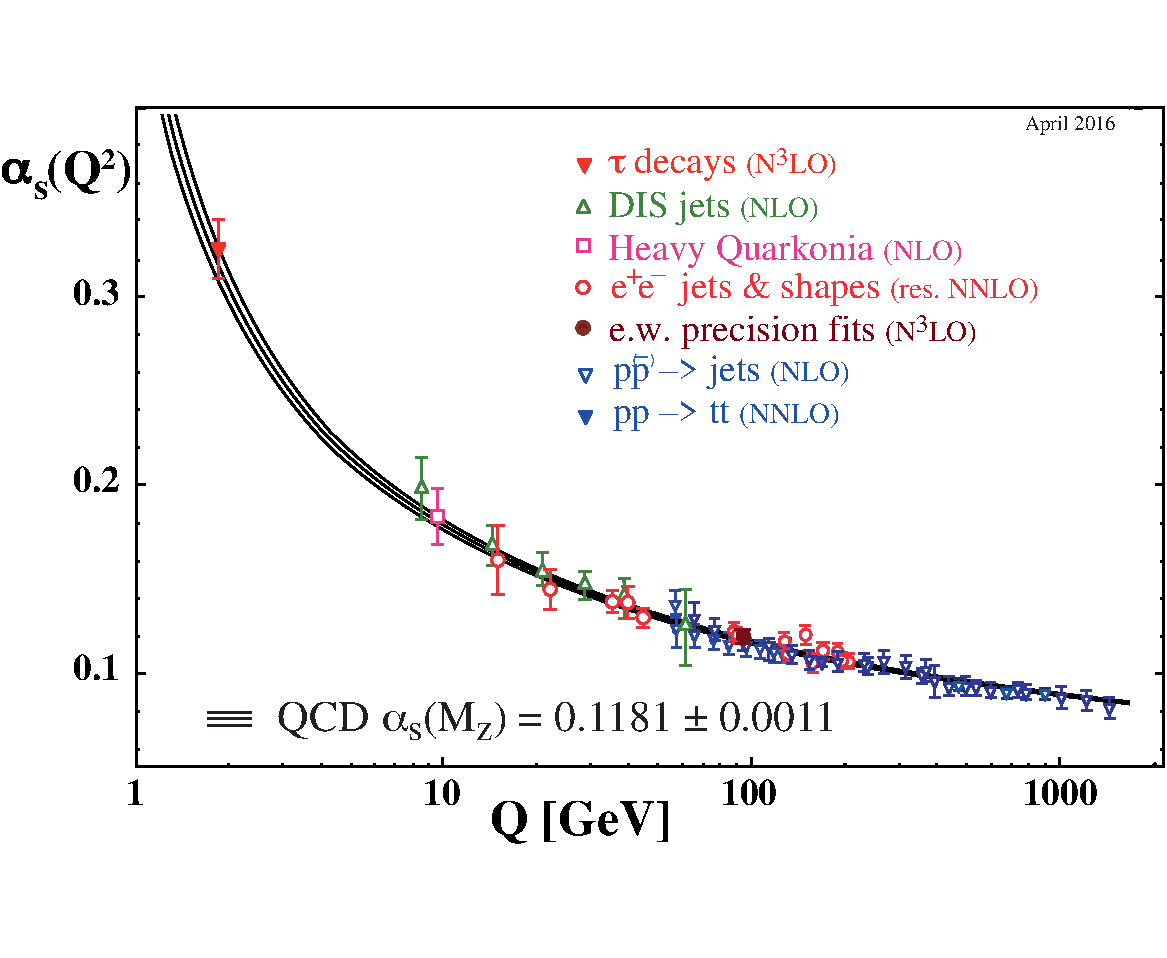
\includegraphics[width=0.8\textwidth]{/Users/Deshan/Documents/PhD/thesis/Thesis/figures/theory/sm/asq-2015.pdf}
    \caption{Summary of experimental measurements of $\alpha_s$ as a function of energy scale Q~\cite{PDG}.}
    \label{fig:alphasrun}
\end{figure}
\subsection{Electroweak symmetry breaking}\label{sec:symmbreak}
As described in the previous sections, the inclusion of explicit mass terms for the fermions and bosons violates the electroweak gauge symmetry. Therefore, the Brout-Englert-Higgs mechanism~\cite{Higgs1964,Englert1964}, commonly referred to as the Higgs mechanism, is used to introduce gauge-invariant mass terms for the particles. A new field is introduced which has gauge-invariant transformations under SU(2)$_\mathrm{L}\otimes\mathrm{U(1)}_\mathrm{Y}$. It can be a complex scalar field in the SM Lagrangian that is an isospin doublet with hypercharge $Y = \frac{1}{2}$, defined as
\begin{equation}\renewcommand*{\arraystretch}{\newarraystrech}
    \label{eq:scalarfield}
    \begin{aligned}
        & \Phi = 
        \begin{pmatrix}
            \phi^+ \\*[0.3cm]
            \phi^0 
        \end{pmatrix} =
        \frac{1}{\sqrt{2}} 
        \begin{pmatrix}
            \phi_1 + i\phi_2 \\*[0.3cm]
            \phi_3 + i\phi_4
        \end{pmatrix}.
     \end{aligned}
\end{equation}
The gauge invariant Higgs Lagrangian is then defined as
\begin{equation}
    \label{eq:lagrangianhiggs}
    \begin{aligned}
        \mathcal{L}_\mathrm{Higgs} &= (D^\mu\Phi)^\dagger(D^\mu\Phi) - V(\Phi), \\
        V(\Psi) &= - \mu^2\Phi^\dagger\Phi + \lambda(\Phi^\dagger\Phi)^2,
     \end{aligned}
\end{equation}
using the covariant derivative defined in \cref{sec:electroweak}, where the potential is given in terms of the free parameters $\mu$ and $\lambda$. For $\mu^2 > 0$ the potential has a minimum at $\phi = 0$, where the minimum corresponds to the vacuum. This corresponds to a Lagrangian with scalar particles of mass $\mu$. However, when $\mu^2 < 0$, the potential has a degenerate minimum at $v = \mu/\sqrt{\lambda}$, where $v$ is the \emph{vacuum expectation value}, and results in spontaneous symmetry breaking. In the potential, the self-coupling parameter $\lambda$ is chosen to be positive to ensure that the potential is bounded from below. The fields are chosen such that $\phi_1 = \phi_2 = \phi_4 = 0$ and $\phi_3 = v + h(x)$. The scalar field, $h(x)$, is identified as the Higgs field. The minimum of the potential after the spontaneous symmetry breaking occurs for the neutral component of the scalar field doublet to preserve U(1) symmetry. The non-zero vacuum expectation value results in the breaking of the SU(2)$_\mathrm{L}\otimes\mathrm{U(1)}_\mathrm{Y}$ symmetry to $\mathrm{U(1)}_\mathrm{EM}$ symmetry. After symmetry breaking, $\Phi$ takes the form 
\begin{equation}\renewcommand*{\arraystretch}{\newarraystrech}
    \label{eq:higgsfield}
    \begin{aligned}
        & \Phi = 
        \begin{pmatrix}
            0\\
            v + h(x)
        \end{pmatrix}.
     \end{aligned}
\end{equation}
Using the Lagrangian in \cref{eq:lagrangianhiggs}, and expanding the kinetic terms, results in a series of terms describing the interactions of the gauge bosons with the vacuum and the Higgs field. This leads to the vector boson masses, 
\begin{equation}
    \label{eq:bosonmasses}
    \begin{aligned}
        m_W &= \frac{gv}{2},\\
        m_Z &= \frac{1}{2}(g^2 + g^{\prime 2})^{\frac{1}{2}}v,
     \end{aligned}
\end{equation}
and the photon remains massless. The masses acquired by the $W^\pm$ and $Z$ gauge bosons are expected by Goldstone's theorem~\cite{PhysRev.127.965}, which states that the vanishing degrees of freedom under SU(2)$_\mathrm{L}$ correspond to Goldstone bosons that are "eaten" to give mass to the associated gauge fields. 

Using the scalar doublet defined in \cref{eq:higgsfield}, fermion masses can also be incorporated. Using the first generation of quarks as an example and defining the SU(2)$_\mathrm{L}$ doublet for left-handed quarks, a Yukawa Lagrangian can be written as, 
\begin{equation}
    \label{eq:YukawaLagrangian}
    \begin{aligned}
        \mathcal{L}_\mathrm{Yukawa} &= -\lambda_d Q_L \Phi d_R - \lambda_u Q_L \tilde{\Phi}u_R + h.c,
     \end{aligned}
\end{equation}
where $\lambda_{d}$ and $\lambda_u$ are the Yukawa couplings of the down- and up-type quarks, respectively. h.c refers to the addition of the Hermitian conjugate of the Higgs doublet. The fermion masses are found to be proportional to the vacuum expectation value of the Higgs field, given by the following relation
\begin{equation}
    \label{eq:fermionmass}
    \begin{aligned}
        m_d = \frac{\lambda_d v}{\sqrt{2}},~~m_u = \frac{\lambda_u v}{\sqrt{2}}.
     \end{aligned}
\end{equation}
% Including all generations of fermions results in non zero Yukawa couplings that mix flavour generations. The resulting matrix can be diagonalised by performing the unitary transformations between the weak- and mass-bases of the fermion fields. This rotation gives rise to \emph{charge-parity} (CP) violation in the charged current interactions, parametrised by the CKM matrix~\cite{10.1143/PTP.49.652} matrix in the quark sector, and the PMNS matrix~\cite{Maki1962} in the leptonic sector.
However, the mass terms for the neutrinos are often omitted from the SM. The inclusion of neutrino mass terms would require an extraordinarily large mass difference between the charged and neutral leptons within each lepton generation. 

Finally, after electroweak symmetry breaking, and the Higgs field acquiring the vacuum expectation value, the Higgs mass is given as
\begin{equation}
    \label{eq:higgsmass}
    \begin{aligned}
        m_h = \sqrt{2\lambda}v.
     \end{aligned}
\end{equation}
In 2012, the SM Higgs boson was discovered with $m_h \sim \SI{125.09}{\giga\electronvolt}$~\cite{Aad_2012,Chatrchyan2012} by the ATLAS and CMS collaborations at CERN. 

